\documentclass[11pt]{article}

% Call the style package
%\usepackage{fun3style}

\title{Quaternion Neural Networks for 3D Sound Source Localization in Reverberant Environments: Implementation using First Order Ambisonics}
\author{Roberto Aureli, ID 1757131\\
		Riccardo Caprari, ID 1743168\\
		Gianmarco Fioretti, ID 1762135}

\date{Neural Networks, Spring 2020}



\usepackage{graphicx}
\usepackage{subfig}

\graphicspath{{./img/}}

\usepackage[utf8]{inputenc}
\usepackage[english]{babel}


\usepackage{xcolor}
\usepackage{nth}
\usepackage{amsmath}
\usepackage{relsize}
\usepackage{wrapfig}
\usepackage{float}
\usepackage{hyperref}
\usepackage{listings}
\usepackage{multirow}

\usepackage{caption}
\usepackage{array}


\usepackage{wrapfig}
\usepackage{csquotes}
\usepackage{float}
\usepackage{amssymb}
\usepackage{multicol}
\usepackage{ragged2e}


\usepackage{indentfirst}

\setlength{\parindent}{2em}
\setlength{\parskip}{1em}

\newcolumntype{P}[1]{>{\centering\arraybackslash}p{#1}}
\renewcommand{\arraystretch}{1.4}


\begin{document}



\maketitle

\vspace{10px}

\openup -2.5ex
\tableofcontents
\openup 2.5ex

\newpage
\section{Introduction}\label{cha:intro}

This project addresses the \textbf{3D Sound Event Localization and Detection Task} in reverberant environments with a  quaternion neural network (deep neural network with quaternion input features extracted from the acoustic intensity vector).\newline

\noindent
As mentioned above, the proposed model performs both sound localization and sound event detection and subsequent classification. In particular it follows the architecture described in paper \cite{paper2020} which allows to estimate the three-dimensional direction of arrivals (DOA), in addition, it has been modified in order to be capable of detecting sound events and estimating the corresponding sources (eleven different classes provided by the development dataset, check for Table \ref{table:classes}).\newline

\noindent
Many recent works have proven that deep quaternion neural networks are able to improve localization performances dramatically, especially in reverberant and noisy environments, thanks to spatial harmonic decomposition which permits to exploit the intrinsic correlation of the ambisonics signal components. One of the main aspect to be considered is the input features to be passed to the network.\newline

\noindent
Our main work consisted in adapting the provided code to the new dataset, fine-tuning the model's hyper-parameters, applying the three metrics defined in a precedent paper \cite{paper2019} (\textbf{SED, DOA, SELD}), implementing the direction of arrival estimation in cartesian coordinates, and computing the confidence intervals on the model's final errors as defined in Perotin et al. paper \cite{paper2018} in order to add also a statistical evaluation on final results.

\newpage
\section{Dataset}\label{cha:data}

The network is trained with the \textbf{TAU Spatial Sound Events 2019 - Ambisonics} dataset which provides four-channel directional microphone array recordings of stationary point sources, with a maximum number of simultaneously overlapping sources equal to 2.\\
It is a balanced dataset, it indeed consists of 11 classes, each with 20 examples randomly split into 5 sets with an equal number of examples for each class. The recordings are synthesized through the collected spatial location impulse responses, at 504 unique combinations of azimuth, elevation and distance triplets.\\
Moreover, in order to improve the performance over new sound events, and to make scenarios more realistic, natural ambient noise collected in the recording locations is added to the synthesized recordings in the dataset.
\newline
\begin{table}[ht]
	\caption{TAU Spatial Sound Events Classes}
	\centering
	\begin{tabular}{c c}
		\hline\hline
		Sound class & Index \\ [0.5ex]
		\hline
		knock & 0 \\
		drawer & 1 \\
		clearthroat & 2 \\
		phone & 3 \\
		keysDrop & 4 \\
		speech & 5 \\
		keyboard & 6 \\
		pageturn & 7 \\
		cough & 8 \\
		doorslam & 9 \\
		laughter & 10\\
		\hline		
	\end{tabular}
	\label{table:classes}
\end{table}

\subsection{Specifications}

The impulse responses obtained in the STFT domain are collected at every $10^\circ$ azimuth angle for 9 different elevation from $-40^\circ$ to $40^\circ$ at 1 meter distance, at first. Then, at every $10^\circ$ azimuth angle for 5 different elevation from $-20^\circ$ to $20^\circ$ at 2 m distance.\\
These impulse responses are recorded in 5 different scenarios (indoor locations) which clearly have different reverberant properties, however, the official specifications do not actually provide them. The 5 scenarios involved are as follows:
\begin{itemize}
	\item Large common area with multiple seating tables and carpet flooring. People chatting and working.
	\item Large cafeteria with multiple seating tables and carpet flooring. People chatting and having food.
	\item High ceiling corridor with hard flooring. People walking around and chatting.
	\item Corridor with classrooms around and hard flooring. People walking around and chatting.
	\item Large corridor with multiple sofas and tables, hard and carpet flooring at different parts. People walking around and chatting.
\end{itemize}

\noindent
The 11 classes comprise 20 examples each, which are split into 5 k-fold splits, four are used for synthesizing the development data set, while the remaining on is used for the evaluation data set. It is divided into four cross-validation split in the development set, which is therefore composed of 400 (100 for each split), one-minute long recordings sampled at 48 kHz, while the evaluation set consists of 100, one-minute long recordings. Each of the recording in these splits is generated randomly. The impulse responses are used from a single location for each sound events in a recording. Moreover, half of the recordings are synthesized with up to 2 temporally overlapping sound events while the others with no overlapping ones. Finally, as already mentioned, the ambient noise collected at the respective location's impulse response is added such that the average SNR is 30 dB for all the sound events.\\
Since the recordings are collected through a microphone array the Ambisonic data set is then obtained by converting the 32 channel microphone signals to First Order Ambisonic ones, by means of encoding filtered based on anechoic measurements of the microphone array response.

\noindent
Summarizing, there are 100 recordings for each split of the dataset, each of them is composed of 10 recordings with up to 2, or no temporally overlapping sound events, synthesized from 5 locations, namely 20 recordings for each location, 10 with overlapping sound events and 10 without. The dataset provided only guarantees a balanced distribution of sound events in each of the azimuth and elevation possible angles, but there's no guarantee about the distribution of locations' impulse responses.

\newpage
\section{Architecture}\label{cha:arch}

The network proposed in the paper \cite{paper2020} involves a series of convolutional layers in the quaternion domains, they are composed of several filter kernels which allow learning inter-channel features, with subsequent activation functions and max-pooling functions. The output of this series are properly reshaped and fed to bidirectional quaternion recurrent layers. This first part of the architecture is depicted in Figure \ref{fig:arch1}

\begin{figure}[ht]
	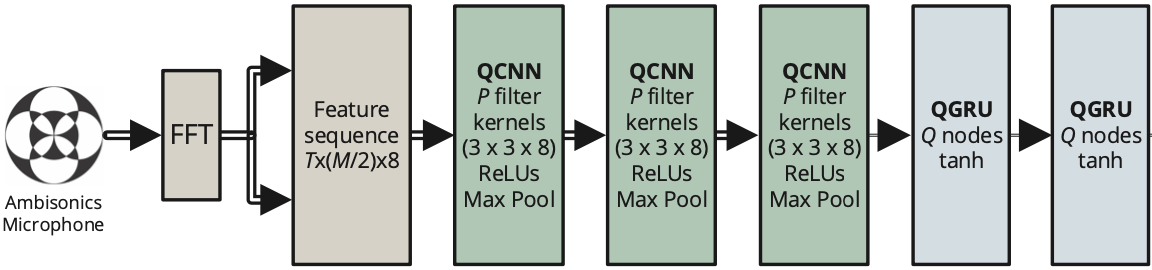
\includegraphics[width=\linewidth]{img/arch1.png}
	\caption{First part of the Network Architecture}
	\label{fig:arch1}
\end{figure}

\noindent
As already pointed out on Chapter \ref{cha:intro} the network has been modified accordingly, the final part of architecture therefore becomes as in Figure \ref{fig:arch2}, so that network is able to perform a multi-classification for the SED task (one for each class: 1 to indicate detection, 0 otherwise) and multi-regressions for DOA task (which has in input azimuth angle, elevation angle, distance and returns cartesian coordinates).

\begin{figure}[ht]
	\centering
	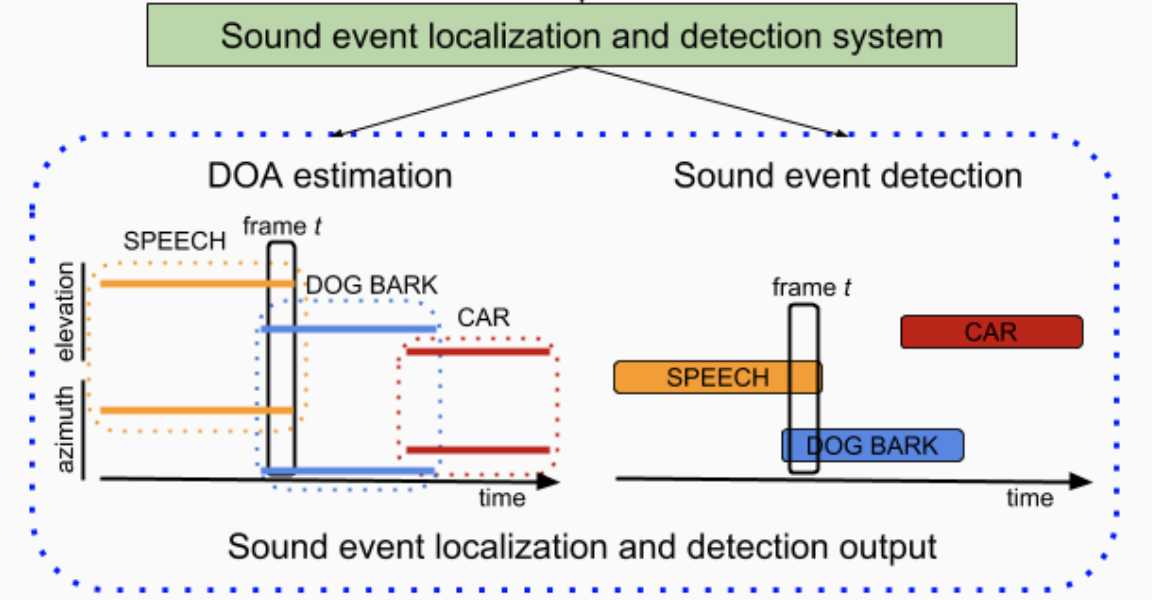
\includegraphics[scale=0.5]{img/arch2.png}
	\caption{Last part of the Network Architecture}
	\label{fig:arch2}
\end{figure}

\newpage
\section{Our work}

The objective of our work is to build a working SELDnet based network that works with First Order Ambisonics data sets. In particular, we are going to extend SELDnet, adding capabilities to both support pre-existing data sets (ansim, resim, etc.) and the FOA one in a smart, modular, performing way. Other metrics have been added like the SELD score, mainly used in the paper \cite{paper2019} outcomes evaluation, and a tiny library for a graphical representation of the results. Now we'll proceed with a more technical analysis of the work, listing all the features added.

\subsection{Project implementation}
We decided to mantain a parameters manager file to configure the SELDnet, which contains for example it's input dataset with specific values, training, evaluation and test process combinations and many other settings that can be found in \textit{parameter.py}. We can divide our project in 3 main classical phases: extraction, training and test. We will cover these three parts after highlighting the main changes on input parameters:

\begin{itemize}
\item \textit{parameter.py}: extension of \textit{quick\_test} parameters supporting now batch and steps size. Support for data sets and extraction output directiories paths. New training management handling different splits also for validation and test evaluation.
\end{itemize}

\subsubsection{Extraction}

Before starting with the training, we have to extract features from the new FOA data set. This delicate process makes the difference between a successful training in terms of evaluation metrics. For this reason we decided to introduce a new \textit{FeatureClass}, which will differ from the old one in some parameters and procedures. In fact, as we experienced, introducing a new similar class results in a way more readable, modifiable and modularizable approach. We noticed, in fact, that different data sets can be similar from a structure point of view and totally different with respect to their parameters, like record settings. For this reason a new full-dedicated extractor results in a wise and faster-implementation choice.

\noindent
As we can observe in scheme \ref{fig:extraction}, \textit{batch\_feature\_extraction.py} has the task of managing the extraction process, differing function calls with respect to data set type. The input is divided into two folders, \textit{foa\_dev} and \textit{metadata\_dev}, which contain audio records stored with a \textit{.wav} format and their corresponding labels.

\begin{figure}[h!]
	\centering
	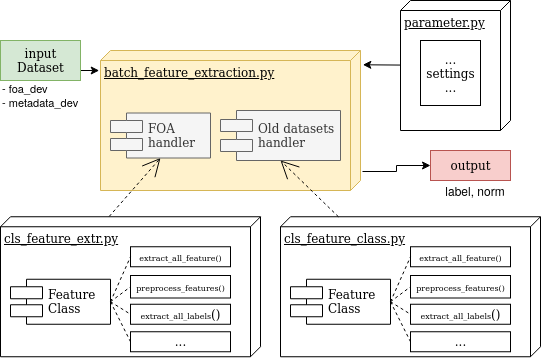
\includegraphics[width=12.5cm]{img/extraction.png}
	\caption{Extraction process.}
	\label{fig:extraction}
\end{figure}

\noindent
Let's now zoom in the new \textit{cls\_feature\_extr.py} extractor and highlight the main differences with the other one. These are the most significant adjustments:

\begin{itemize}
	\item \textit{FeatureClass()}: changes on hop length, which are the number of audio samples between adjacent STFT columns; win length, which windows each audio frame by a certain number; nfft has been changed and chosen to fit win length taking the next greater power of 2; new data set output folder management.
	\item \textit{spectrogram()}: use of \textit{librosa} library for the short-time Fourier trasform taking a cue from \cite{git}. Then we cycled over the number of channels to get the stft and transpose it to compose the final spectra. After, we loaded each audio file, extracted its spectogram and subsequently saved in a \textit{.npy} format.
	\item \textit{preprocess\_features()}: use of \textit{StandardScaler} which is in charge of standardizing the features. Adding partial fit of the scaler in order to compute mean and std of the precedent computed feature files.
	\item \textit{extract\_all\_labels()}: weakness and mode parameters have been remove; slight edit on get labels process.
\end{itemize}

\noindent
After the extraction has been done we will deal with three new different folders inside \textit{/feat\_label\_tmp}, which contain \textit{.npy} files. Here is a list of them: 

\begin{itemize}
	\item \textit{foa\_dev\_label}: storing labels.
	\item \textit{foa\_dev\_norm}: which stores normalized features.
	\item \textit{foa\_dev}: which stores unnormalized features.
\end{itemize}



\subsubsection{Training}\label{minisec:train}

After the process of features extraction is completed we can proceed with the training. Unlike for the extraction, in this phase we introduced some changes to both manage foa data sets and old ones instead of adding a completely new \textit{seld.py}. In particular, we highlight differences on:

\begin{itemize}
	\item \textit{cls\_data\_generator.py}: new split handler system, in \textit{\_get\_label\_filenames\_sizes()} we added support for train and validation$/$test splits which has as objective to create a correct file list, depending also from the new ov number in the constructor. All the files are now taken according to \textit{parameter.py} settings, which specify the number of the splits. Adding check control for circular buffers in generator's \textit{generate()} base function in case pop operations exceed buffer size.
	\item \textit{seld.py}: new batch and step control for quick tests; changing \textit{unique\_name} for model weights data saving; new smart resumption of training if weights are present in \textit{/model} folder; new important \textbf{bug-solving} procedure to let \textit{predict\_generator()} work correctly, which consists of creating the model, save it and reload it with old weights before a prediction occurs; new confidence interval calculator for DOA and SED errors; adding SELD to the scores and saving all of them in a csv file.
	\item \textit{evaluation\_metrics.py}: adding \textit{compute\_confidence()} and\\ \textit{compute\_doa\_confidence()}, functions to compute 95\% confidence interval given an array of data. Implementation based on \cite{confint}.
	\item \textit{simple\_plotter.py}: new file which can be used for csv saving, metrics 2D plotting and data prediction 3D plotting.
\end{itemize}

\begin{figure}[h!]
	\centering
	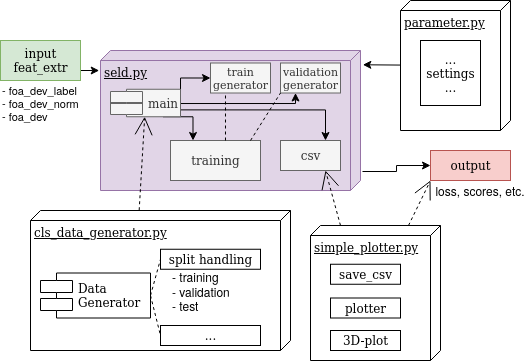
\includegraphics[width=13.5cm]{img/training.png}
	\caption{Training process.}
	\label{fig:training}
\end{figure}

\noindent
In figure \ref{fig:training} it's possible to have a general view of \textit{seld.py} in action. During the training we fit the model using a data train set and then, for each epoch, we use another smaller set as validation to compute all the necessary metrics. These metrics are then saved in a csv file in a consecutive way, meaning that each line corresponds to an epoch. Then, apart from \textit{seld.py}, we generate all the plots which will be discussed in Chapter \ref{cha:res}.

\newpage
\subsubsection{Test}

Finally, we end up with test phase. This part wasn't really handled from the original code so we decided to add it to have a full final evaluation of a different set. In fact, by adding a new split in \textit{parameter.py}, we are able to load weights of a pre-trained model and then make a full test using it. This part, like for the training one, includes all the evaluation metrics, confidence intervals and plots making.

In particular, the new included file for testing is \textit{seld\_test.py}. This program involves the creation of a new model whose weights are loaded from a trained one, two data generators (train + test) and a single prediction using \textit{Keras} library.


\subsubsection{Summary}

Recapping, this is an overview of the introduced and changed files:

\begin{tabular}{cp{0.6\textwidth}}
  New:\\  
  $+$ & batch\_feature\_extr.py \\
  $+$ & simple\_plotter.py \\
  $+$ & seld\_test.py \\
  \\
  Changed:\\
  $\thicksim$ & parameter.py\\
  $\thicksim$ & batch\_feature\_extraction.py\\
  $\thicksim$ & cls\_data\_generator.py\\
  $\thicksim$ & seld.py\\
  $\thicksim$ & evaluation\_metrics.py\\
  \\
  Removed:\\
  $---$ 
\end{tabular}\\


\newpage
\section{Results}\label{cha:res}

The First Order Ambisonics data set we are going to use is divided into four different splits. As suggested by the dataset documentation, for keeping a certain uniformity in the results, the folds for the k-fold validation procedure are standardized. The four sets proposed in Table \ref{table:folds} are composed of training, validation and testing split.  
To recover information about how the network performs in the various situations presented, the test phase will be performed separately for sound overlaps, resulting in two sets of outcomes.

\begin{table}[h]
\caption{Proposed splits for the k-fold procedure.}
\begin{center}
\begin{tabular}{l|lll}

Folds  & \multicolumn{1}{l|}{Training splits} & \multicolumn{1}{l|}{Validation split} & Testing split \\ \hline

Fold 1 & 3,4                                  & 2                                     & 1             \\

Fold 2 & 4,1                                  & 3                                     & 2             \\

Fold 3 & 1,2                                  & 4                                     & 3             \\
 
Fold 4 & 2,3                                  & 1                                     & 4            
\end{tabular}
\end{center}
\label{table:folds}
\end{table}

\noindent
We decided to use Fold 1 for the training process, validation and a final test. In order to obtain substantial results we trained the model for 100 epochs with a \textit{batch\_size} equal to 16 using \textit{Tesla K80} GPU from Google Colab.

\noindent
Initially, we were obtaing results with a really low accuracy even after plenty of epochs. This was caused by a Keras bug related to the use of \textit{fit\_generator()} and \textit{predict\_generator()} functions. However, we managed to solve this as explained in training part (\ref{minisec:train}). 

\noindent
We present, through different plots, the results obtained using this specific combination of splits and the new implementation of the project. The first analysis we are going to conduct is the loss function. In Fig. \ref{fig:loss} it's possible to see how training and validation loss decrease almost monotonically. The gap between the two functions is really small in the first 30/40 epochs and tends to grow in the second part. However, we can say that overfitting is relatively small and doesn't influence results in a particular way.

\begin{figure}[h!]
	\centering
	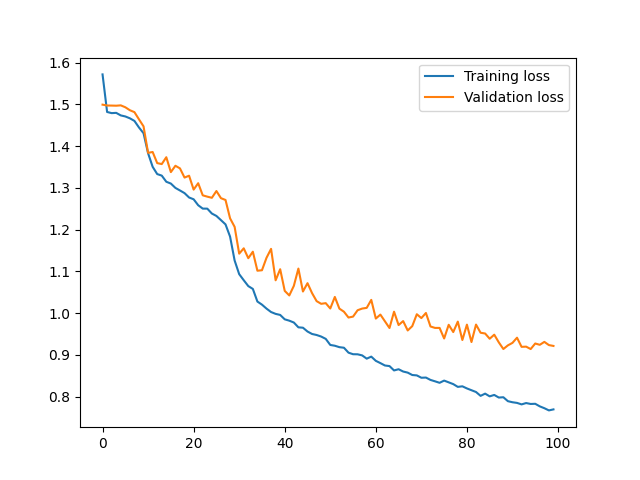
\includegraphics[width=10cm]{img/loss.png}
	\caption{Loss function over 100 epochs.}
	\label{fig:loss}
\end{figure}

\noindent
A second plot we decided to produce and comment out is the one showing the main scores over the epochs. Specifically, these scores are DOA (Direction Of Arrival), SED (Sound Event Detection) and SELD (Sound Event Localization Detection). We compute them as:

$S_{SED} = \frac{ER + (1-F)}{2}$ \space\space
$S_{DOA} = \frac{\frac{DOA_{err}}{180} + (1-K)}{2}$ \space\space
$S_{SELD} = \frac{S_{SED} + S_{DOA}}{2}$ \space\space

\noindent
in which $ER$ is the SED error rate and $F$ is the f1-score; $DOA_{err}$ is the DOA estimation error and $K$ is the recall which takes into account true positives.

Observing Fig. \ref{fig:scores} and Fig. \ref{fig:erf1} it's possible to see the behavior of the scores with the addition of F and ER SED's terms over 100 epochs. In the almost first 10 epochs the error rate ER is fixed to 1 which means that the model is predicting wrong with a percentage of 100\%. On the other hand, f1-score is obviously fixed to zero because of the completely wrong predictions. These two terms results in an overall SED score fixed to one. In fact, the smaller these scores results the better they are. We can notice that as soon ER and F moves respectively from 1 and 0, SED scores starts to decrease rapidly.

\begin{figure}[h!]
	\centering
	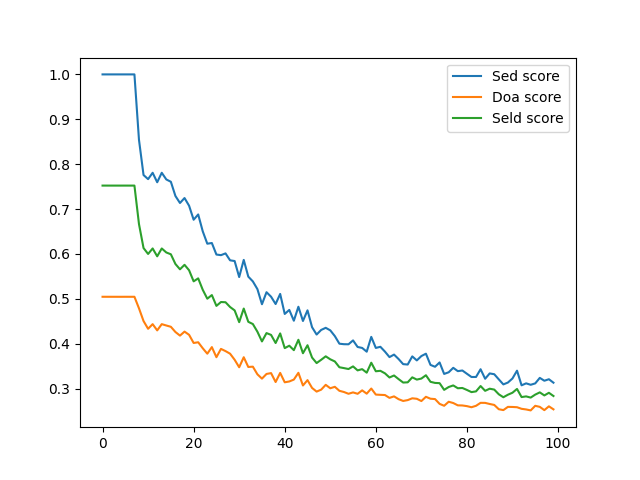
\includegraphics[width=10cm]{img/scores.png}
	\caption{Sed, Doa and Seld scores over 100 epochs.}
	\label{fig:scores}
\end{figure}

\newpage
\begin{figure}[h!]
	\centering
	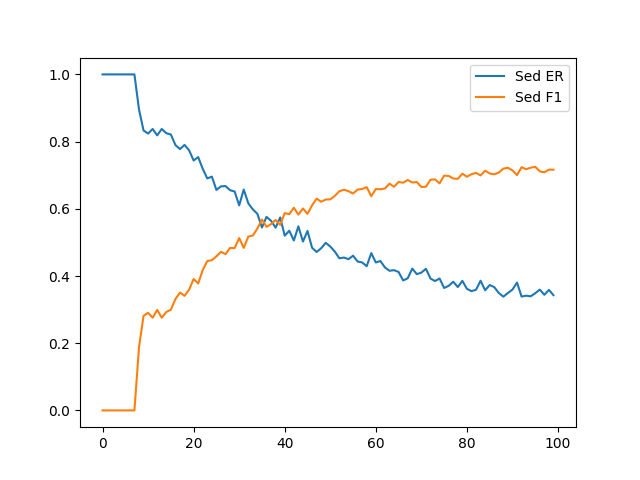
\includegraphics[width=10cm]{img/er_f1.png}
	\caption{Sed error rate and f1-score over 100 epochs.}
	\label{fig:erf1}
\end{figure}

\noindent
This overview is the same for DOA score which starts with a value of 0.5 and starts to decrease in a same fashion. Due to that SELD will behave in the same way, being an average of the precedent two scores.

\noindent
We finally ended up with these training scores:

\begin{center}
\begin{tabular}{cp{0.6\textwidth}}
$S_{DOA} = 0.31$ \space\space $S_{SED} = 0.25$ \space\space $S_{SELD} = 0.28$
\end{tabular}
\end{center}

\noindent
After a full training we decided then to test the remaining split (1) using the new \textit{seld\_test.py} program. We evaluated this split distinguishing overlaps. In fact, the splits, which size is 100, are perfectly balanced, having 50 samples of OV1 and OV2. In Table \ref{table:scores} we report outcomes evaluated with several evaluation metrics.
\newline

\begin{table}[h]
\centering
\caption{Scores obtained during the test.}
\begin{tabular}{ |P{3cm}||P{3cm}|P{3cm}|  }

 \hline
 \multicolumn{3}{|c|}{Final outcomes} \\
 \hline
 Metric & OV1 & OV2\\
 \hline
 precision & 0.78 & 0.83\\
 recall & 0.78 & 0.62\\
 $S_{DOA}$ & 0.156 & 0.315\\
 $S_{SED}$ & 0.219 & 0.329\\
 $S_{SELD}$ & 0.187 & 0.322\\
 SED error 95\% confidence interval & [0.216922, 0.221115] & [0.371710, 0.376616]\\
 \hline
\end{tabular}
\label{table:scores}
\end{table}

In Fig. \ref{fig:conf_int} we propose also a graphic visualization of 95\% confidence intervals for DOA error. All the 95\% confidence intervals we calculated are relatively small, meaning that there is a small uncertainty.


\begin{figure}[!tbp]
  \centering
  \subfloat[OV1]{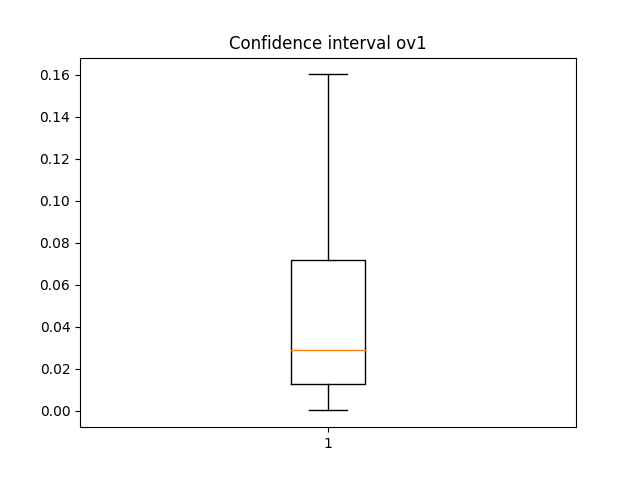
\includegraphics[width=0.5\textwidth]{confidence_int_ov1.png}\label{fig:ov1}}
  \hfill
  \subfloat[OV2]{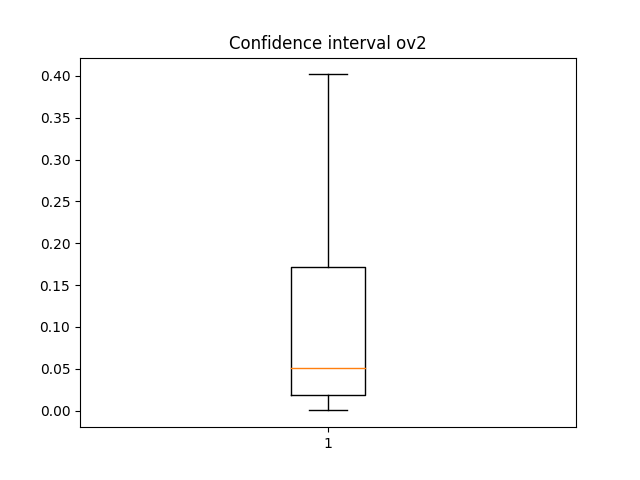
\includegraphics[width=0.5\textwidth]{confidence_int_ov2.png}\label{fig:ov2}}
  \caption{$DOA_{err}$ 95\% confidence intervals.}
  \label{fig:conf_int}
\end{figure}




\newpage
\noindent
With the precedent results we decided to introduce a new tool to better visualize and understand in a geometric way what is really happening: 3D-plotting. Using predictions from \textit{predict\_generator()}, we made a comparison with ground truth values, finding a spatial meaning for our results. In particular, we used random sampling in both pred and gt sets to give a better look on what's happening (plotting thousand of points may look terrible and counterintuitive). To be exact, we chose 200 points per class.

\noindent
In Fig. \ref{fig:plot_doa} there is a first 3D-plot for DOA predictions, which are placed on the left. On the right it's possible to see how ground truth points are affected by the presence of outliers, which are not always well predicted by the model and, by the fact, suffers from. Further observing, it seems that the number of points in the two frames is different: this is just a perception due to the fact that many ground truth points overlap while those on the left are badly predicted.



\newpage
\begin{figure}[h!]
	\centering
	\hspace*{-2.5cm}
	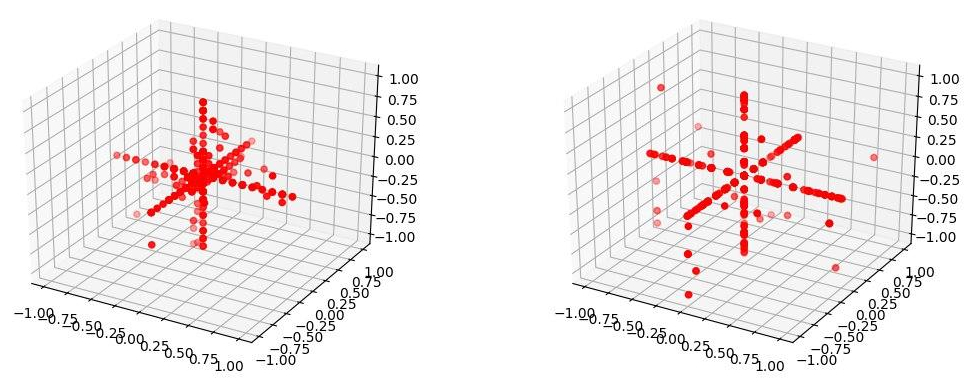
\includegraphics[width=17.7cm]{img/plot_doa.jpg}
	\caption{(Left) DOA prediction points \\ \hspace{1cm} (Right) DOA ground truth points}
	\label{fig:plot_doa}
\end{figure}

\begin{figure}[h!]
	\centering
	\hspace*{-2.5cm}
	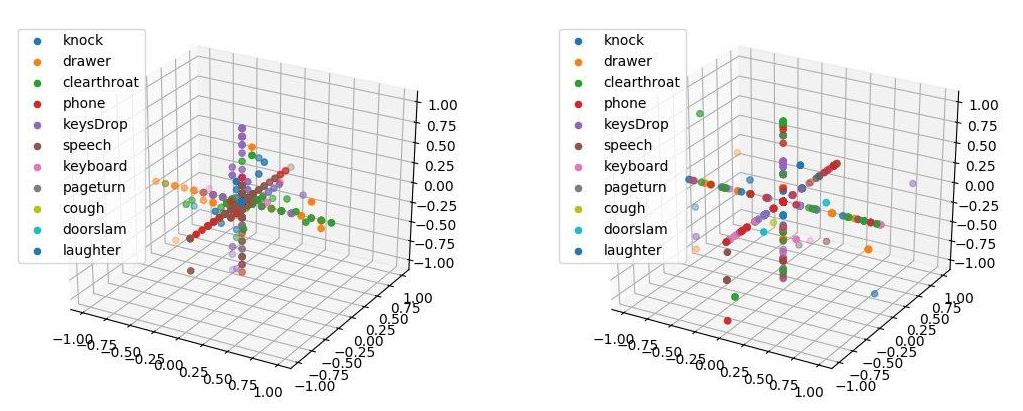
\includegraphics[width=17.7cm]{img/plot_labels.jpg}
	\caption{(Left) SELD prediction points\\ (Right) SELD ground truth points}
	\label{fig:plot_labels}
\end{figure}

\newpage
\begin{figure}[h!]
	\centering
	\hspace*{-2.5cm}
	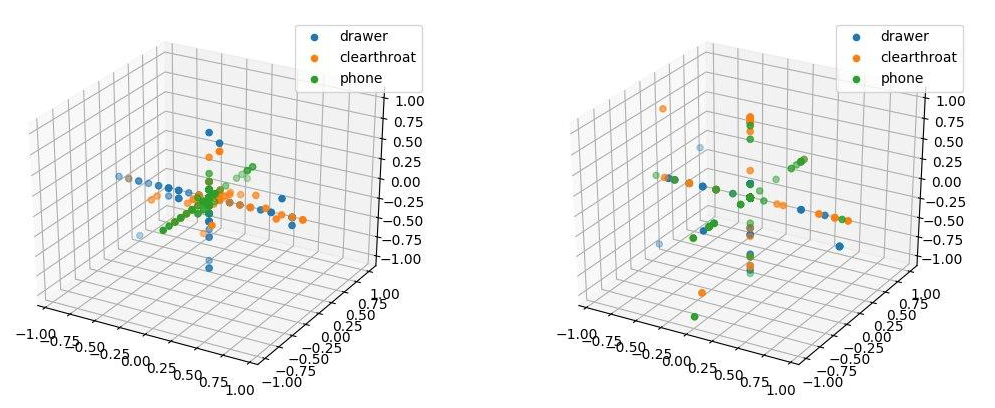
\includegraphics[width=17.7cm]{img/plot_3labels.jpg}
	\caption{(Left) SELD prediction points for 3 classes\\ (Right) SELD ground truth points for 3 classes}
	\label{fig:plot_3labels}
\end{figure}


\noindent
We made then other two plots, Fig. \ref{fig:plot_labels} and Fig. \ref{fig:plot_3labels}, which are the combination of DOA and SED. In the first one all the classes have been plotted to get a total overview and behaviour of the network. The second one refers to 3 classes only to better understand predictions in a smaller set of points.

\newpage
\section{Conclusion}\label{cha:conc}

Main objective of this work was to let the SELDnet project work with different type of data sets, in particular the First Order Ambisonics TAU Spatial Sound Events 2019. We managed to deal with it starting from three main papers (\cite{paper2020}, \cite{paper2019}, \cite{paper2018}) and understanding how SELDnet works.

\noindent
We tried not to find the easiest solution but one of the most optimized and better-performing ones. We proceeded with a technical analysis of the code and a training process to allow us producing valid results. In the second part, we presented different plots of our outcomes to realize and comment out how the network is performing. 

\noindent
We consider ourselves satisfied with the results obtained. We didn't deal with a specific study of the network and its architecture but we leave this as future work.


\newpage
\begin{thebibliography}{999}

\bibitem{paper2020}
  Michela Ricciardi Celsi, Simone Scardapane and Danilo Comminiello,
  \emph{Quaternion Neural Networks for 3D Sound Source
Localization in Reverberant Environments},
  DIET Dept., Sapienza University of Rome,
  2020.

\bibitem{paper2019}
  Danilo Comminiello, Marco Lella, Simone Scardapane, and Aurelio Uncini,
  \emph{Quaternion Convolutional Neural Networks
For Detection And Localization Of 3D Sound Events},
  DIET Dept., Sapienza University of Rome,
  2019.

\bibitem{paper2018}
  Lauréline Perotin, Romain Serizel, Emmanuel Vincent and Alexandre Guérin,
  \emph{CRNN-based multiple DoA estimation using Ambisonics
acoustic intensity features}, Submited to the IEEE Journal of Selected
Topics in Signal Processing, Special Issue on Acoustic S.. 2018.
  
\bibitem{git}
  \href{https://github.com/sharathadavanne/seld-dcase2019}{Seld-dcase2019} (Link)
  
\bibitem{confint}
  \href{https://www.mathsisfun.com/data/confidence-interval.html}{Confidence Intervals} (Link)

\end{thebibliography}

\end{document}
